% 
\begin{table}[t!]
\centering
{
\footnotesize
\setlength{\tabcolsep}{0.5em}
\rowcolors{2}{lightgray}{white}
\begin{tabular}{l|ccc|ccc}
\toprule
& \multicolumn{3}{c}{Depth metrics} & \multicolumn{3}{c}{3D AP} \\ 
\multirow{-2}{*}{Depth net} & 
Abs Rel$\downarrow$ &
Sq Rel$\downarrow$ &
RMSE$\downarrow$&
Easy$\uparrow$ & Med$\uparrow$ & Hard$\uparrow$ \vspace{0.5mm}\\
\midrule
PackNet~\cite{guizilini20203d}  & 
0.112 & 
0.761 &  
4.756 &  
18.50 &  
12.68 &  
10.78 \\
% BTS~\cite{lee2019big} & 
% 0.116 & 
% 0.935 &  
% 0.210 &  
% 0.842 &  
% 0.945 &  
% \textbf{0.977}\\
PSMNet~\cite{chang2018pyramid} & 
0.043 & 
0.390 &  
2.861 &  
64.83 &  
42.74 &  
34.75\\

\bottomrule
\end{tabular}\\\vspace{0mm}
\caption{
\textbf{3D detection performance on the KITTI3D dataset~\cite{geiger2012we} with different depth inputs.} Packnet~\cite{guizilini20203d} computes depth from monocular images, while PSMNet~\cite{chang2018pyramid} computes depth from stereo. The depth metrics are computed against Velodyne lidar scans on the KITTI3D validation set. The 3D detection numbers are computed using the $AP|_{40}$ metric on the \textit{Car} category of the KITTI3D validation set.}
\label{table:baseline_depth_detection}
}
\end{table}


The goal of 3D object detection from monocular images is the recovery of a function $f_{3D}: I \to \mathbb{R}^{K\times8}$ that identifies $K$ objects in 3D space, parameterized by their 3D position, 3D shape, class and confidence $\left(x,y,z,w,l,h,c,\gamma\right)$. Accurately regressing object position is by far the most challenging task~\cite{manhardt2019roi,simonelli2020demystifying}.  Intuitively, monocular depth estimation and monocular object detection are linked; in this work we dive deeper and establish a clear correlation between the two. We thoroughly test our hypothesis following two leading 3D detection paradigms: (i) \textit{Pseudo-Lidar} (PL) methods~\cite{you2019pseudo,vianney2019refinedmpl,qian2020end,ma2020rethinking}, where depth estimation is an intermediate task with the resulting point cloud being consumed as input by a 3D detector; and (ii) single stage methods~\cite{tian2019fcos,liu2020smoke} that directly regress object properties for each pixel, where we propose a novel \textit{Fully Convolutional} architecture (FCOS-3D)  that combines dense depth estimation and dense object detection.



\subsection{FCOS-3D}
FCOS-3D is a single-stage network that extends FCOS~\cite{tian2019fcos} to perform 3D detection and dense depth prediction. It is composed of backbone network and three \emph{subnetworks}. As in \cite{tian2019fcos}, we adopt feature pyramid network(FPN)~\cite{} 
\begin{figure}[h]
	\centering
	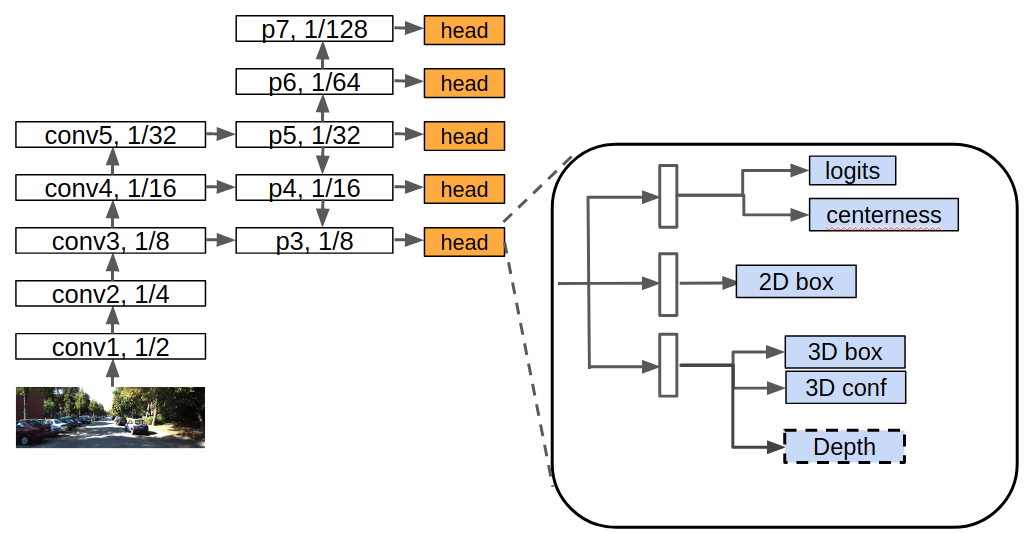
\includegraphics[width=1.0\columnwidth]{figures/fcos3d_arch.png}
	\caption{FCOS-3D extends FCOS to perform 3D detection and dense depth prediction. As in FCOS, a shared head is applied to all levels of FPN features, but with one exception: the depth head is only applied on to the highest resolution features (i.e. $\texttt{p3}$ features).}
\end{figure}

\begin{itemize}
    \item FCOS3D extends FCOS to predict 3D bounding box, in addition to category labels and 2D bounding box.
    \item The output of 3D box head consists of projected centroid, depth of centroid, and size of the 3D box.
    \item Backbone: DLA-34
    \item Matching: Given a 2D bounding box of a foreground object, we associate the features that are within $R$ pixels from the center of 2D bounding box with the given instance.
    \item Loss function: We use disentangled 3D box loss introduced in MonoDis.
    \item 3D confidence: As in MonoDis, we use the 3D confidence, predicted by an additional head, to reweight the logit-based classification score
\end{itemize}

\subsection{Depth pretraining for FCOS-3D}
Dataset: IODA dataset consist of 3.4M pairs or image and Lidar pointcloud. The dataset covers diverse urban environment across US and Japan. The pointcloud is captured by high-resolution Luminar device.
\begin{itemize}
    \item We extend FCOS-3D to perform dense prediction task by aggregating the output of conv2D layer of 3D box head. That is, we upsample all low-resolution features, and add them to produce a dense (stride=4) feature map, and compute depth estimation.
    \item Loss function: we investigate various loss functions, and conclude L1-loss works best. 
    \item Range-aware pretraining. The most challenging instances in monocular 3D detection are in 20-40m range. Therefore, we investigate whether focusing on this range of depth in pretraining helps.
    \item Scale law: We investigate how much of image-pointcloud pairs are needed for a good transfer.
\end{itemize}
\subsection{Depth fine-tuning for FCOS-3D}
\begin{itemize}
    \item Once pretrained, we fine-tune FCOS-3D in multi-task framework, using KITTI3D dataset.
    \item We project Lidar points onto image plane, and use the same archiecture for pretraining to predict sparse per-pixel depth, in addition to the original FCOS-3D losses.
\end{itemize}


\subsection{Pseudo-Lidar 3D detection}
\label{subsec:pseudo-lidar}
PL methods consist of two stages: first, leveraging dense depth estimators, a point cloud is computed given an input RGB image; second, a 3D detector consumes the generated point cloud, outputting detections. The modularity of the PL pipeline implies that any depth estimation method can easily be combined with any detector that consumed point cloud data as input. Moreover, this paradigm allows easy introspection of both components, permitting us to quantify how changes in one affects performance in the other. 

\subsubsection{Monocular depth estimation}
\label{subsubsec:monodepth}

The aim of monocular depth estimation is the recovery of a function $f_D: I \to D$ that predicts for each pixel $p \in I$ the estimated depth $\hat{D} = f_D\left( I\left(p\right)\right)$. Given ground truth depth measurement $D$ (typically acquired by an external sensor, e.g. a LiDAR or RGB-D camera), we define a loss aimed at minimizing the error between the predicted and the actually depth. Formally, our depth estimation model $f_D$ and parameterized by $\theta_D$ is defined as $\hat{\theta}_D = \argmin_{\theta_D}\mathcal{L}_{D}\left(D,\hat{D}\right)$. In all our experiments we 

% \begin{equation} \label{eq:supervised_depth}
% 
% \end{equation}


We supervise our predictions using the scale invariant error proposed by~\cite{eigen2014depth}:  

\begin{equation} \label{eq:silog_loss}
\small
\mathcal{L_D}(D, \hat{D}) =
\frac{1}{N} \sum_{d \in D} e ^2 - \frac{\lambda}{N^2} \left(\sum_{d \in D} e \right)^2
\end{equation}

\noindent where $e$ denotes the error in log space between the predicted and actual depth, $e = \log \hat{d} - \log d$. We follow~\cite{lee2019big} and set $\lambda=0.85$ in all our experiments. We experiment with the PackNet~\cite{guizilini20203d} state-of-the-art network architectures: (i) which uses packing and unpacking blocks with 3D convolutions, allowing it to recover fine structures with high precision; and (ii) BTS~\cite{lee2019big} which leverages local planar guidance layers at different levels allowing better correlation between encoded features and desired output depth  for all our experiments we use the \textit{densenet161} backbone.

% Formally, our depth estimation model $f_D$ and parameterized by $\theta_D$ is defined as: 

% \begin{equation} \label{eq:supervised_depth}
% \hat{\theta}_D = \argmin_{\theta_D}\mathcal{L}_{D}\left(D,\hat{D}\right)
% \end{equation}

% \noindent{\textbf{Loss function.}} We supervise our predictions using the scale invariant error proposed by~\cite{eigen2014depth}:  

% follow~\cite{eigen2014depth} and supervise our predictions using the scale-invariant loss 

% through the Scale Invariant Logarithmic Loss function (SILog) defined as:

% error in log space $\Delta d = \log d - \log \hat{d}$:
% \begin{equation} \label{eq:silog_loss}
% \small
% \mathcal{L_D}(D, \hat{D}) =
% \frac{1}{N} \sum_{d \in D} e ^2 - \frac{\lambda}{N^2} \left(\sum_{d \in D} e \right)^2
% \end{equation}

% \noindent where $e$ denotes the error in log space between the predicted and actual depth, $e = \log \hat{d} - \log d$. We follow~\cite{lee2019big} and set $\lambda=0.85$ in all our experiments.

% \noindent{\textbf{Network architecture.}} We experiment with two state-of-the-art network architectures: (i) PackNet~\cite{guizilini20203d} which uses packing and unpacking blocks with 3D convolutions, allowing it to recover fine structures with high precision; and (ii) BTS~\cite{lee2019big} which leverages local planar guidance layers at different levels allowing better correlation between encoded features and desired output depth  for all our experiments we use the \textit{densenet161} backbone.

% this is particularly relevant for PL methods~\cite{ma2020rethinking,simonelli2020demystifying,qi2018frustum} that leverage an off-the-shelf 2D detector, and perform 3D detection only on image patches where objects have been detected. 

% \noindent{\textbf{Guided training.}} Supervised training of depth estimation network applies the same amount of weight to all supervision points. However, we primarily interested in recovering depth on objects, with depth on other surfaces being less relevant. We follow standard PL~\cite{ma2020rethinking,simonelli2020demystifying,qi2018frustum} practices and assume the availability of an off-the-shelf 2D detector, which we use to detector regions of interest (i.e. objects) in the images. Inspired by keypoint regression methods, we define a mask around object centers, denoted by $\mathcal{M}_{obj}$. We use a Gaussian kernel to associate a weight with each pixel depending on its distance from the object center (see Fig.~\ref{fig:object_masks}). 

% \begin{figure}[h!]
% 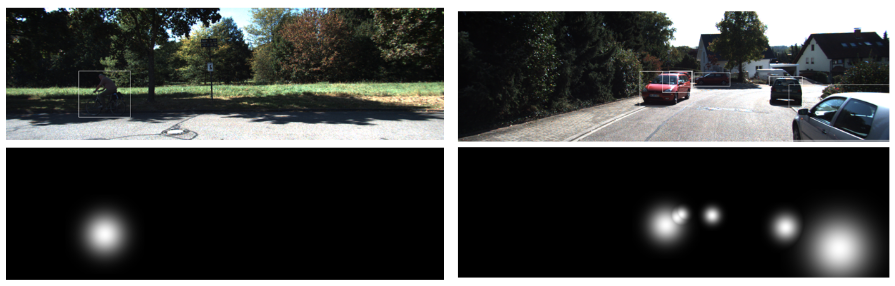
\includegraphics[width=\columnwidth]{figures/object_masks.png}
% \caption{\textbf{Proposed guiding masks for supervised monocular depth training.}}
% \label{fig:object_masks}
% \end{figure}

% We leverage the object masks while training the depth estimation network, and adjust our supervision loss to:

% \begin{equation} \label{eq:masked_silog_loss}
% \small
% \mathcal{L_{MD}}(D, \hat{D}) = \mathcal{L_D}(D, \hat{D}) \circ \mathcal{M}_{obj}
% \end{equation}

% \noindent where $\circ$ to denotes element-wise multiplication. We show in our experiments that the proposed depth guided training scheme improves depth in crucial image regions, leading to improved 3D object detection. 

% \noindent{\textbf{Dataset bias.}} PL methods leverage monocular 3D detectors trained in the same domain. Overlaps in training / validation splits between the two tasks may lead to corrupted results. In the case of the KITTI~\cite{geiger2012we} dataset, the \textit{Eigen train/val} splits proposed in~\cite{eigen2014depth} and commonly used for supervised depth  training~\cite{packnet-semisup,lee2019big,fu2018deep}, overlap with the training and validation set of the KITTI 3D dataset, as described in~\cite{simonelli2020demystifying}. Following~\cite{simonelli2020demystifying}, we remove all overlapping images and generate a new split which we refer to as \textit{Eigen clean}. This procedure is described in more detail in Sec.~\ref{sec:experiments} as well as the supplementary; we will make the new split public to facilitate the generation of unbiased results. We mention that \textit{the depth used by our PL 3D detectors is always trained on Eigen clean, and not on Eigen train}, to avoid any contamination. 



\subsubsection{3D detection}
\label{subsubsec:pl_3d_det}

Our Pseudo-Lidar monocular 3D detector follows the method proposed by~\cite{qi2018frustum,ma2020rethinking}. Given an input image $I$, we predict dense per pixel depth which is converted to a point cloud using the camera intrinsics $K$. For each image pixel $p \in I$ and predicted depth $\hat{d}$, we compute associated 3D point $P$ through: $P=K^{-1}\left[p_x, p_y, \hat{d}\right]$. The point cloud is concatenated with the input image, resulting in a 6D tensor encompassing pixel color values along with 3D coordinates. Leveraging an off-the-shelf 2D detector, proposal regions are identified in images and are fed to a 3D detection network that outputs bounding box parameters. 

\noindent{\textbf{Backbone, detection head and 3D confidence.}}
We follow~\cite{ma2020rethinking}, and process each RoI with a ResNet-18~\cite{he2016deep} backbone that uses Squeeze-and-Excitation layers~\cite{hu2018squeeze}. As the RoI contains both object as well as background pixels, the resulting features are filtered via a foreground/background mask computed based on the associated RoI depth map~\cite{ma2019accurate}. The detection head follows~\cite{ma2020rethinking} and operates in 3 distance ranges, outputting one bounding box for each range; the final output is then selected based on the mean depth of the input RoI. Following~\cite{simonelli2019disentangling,simonelli2020demystifying}, we modify the detection head and also output a 3D confidence value $\gamma$ per detection, which is linked to the 3D detection loss (the architectural details are described in the supplementary).

\noindent{\textbf{Loss function.}} Following~\cite{qi2018frustum} the 3D regression loss is defined as:

\begin{equation} \label{eq:3D_bbox_loss}
\small
\mathcal{L}_{3D} = \mathcal{L}_{center} +  \mathcal{L}_{size} +  \mathcal{L}_{heading} +  \mathcal{L}_{corners}
\end{equation}

We define an additional loss that links the predicted 3D confidence $\gamma$ with the 3D box coordinates loss~\cite{simonelli2019disentangling} using a Binary Cross Entropy (BCE) formulation with target $\hat{\gamma}=e^{-\mathcal{L}_{corners}}$. The final PL 3D detection loss is:

\begin{equation} \label{eq:3D_bbox_loss}
\small
\mathcal{L}_{PL} = \mathcal{L}_{3D} +  \mathcal{L}_{conf}
\end{equation}
